\documentclass[10pt,a4paper]{article}

\newcommand{\AuthorName}{Nicola Rota -- Matricola 10906471}
\newcommand{\InstitutionName}{Politecnico di Milano}
\newcommand{\TutorName}{Carlo Alberto Bono}

\usepackage[utf8]{inputenc}
\usepackage[T1]{fontenc}
\usepackage[italian]{babel}
\usepackage{lmodern}
\usepackage{microtype}
\setlength{\emergencystretch}{2em}
\usepackage{geometry}
\geometry{margin=1.7cm}
\setlength{\columnsep}{0.7cm}
\usepackage{booktabs}
\usepackage{tabularx}
\usepackage{threeparttable}
\usepackage{siunitx}
\sisetup{output-decimal-marker={,}, group-separator={.}, group-minimum-digits=4, group-digits=integer}
\usepackage{amsmath}
\usepackage{graphicx}
\usepackage{caption}
\captionsetup{font=footnotesize,labelfont=bf}
\usepackage{subcaption}
\usepackage{placeins}
\usepackage[table]{xcolor}
\definecolor{linkblue}{HTML}{1F4E79}
\usepackage{csquotes}
\usepackage[colorlinks=true,linkcolor=linkblue,citecolor=linkblue,urlcolor=linkblue]{hyperref}
\usepackage[noabbrev,nameinlink]{cleveref}
\crefname{figure}{figura}{figure}
\Crefname{figure}{Figura}{Figure}
\crefname{table}{tabella}{tabelle}
\Crefname{table}{Tabella}{Tabelle}
\crefname{section}{sezione}{sezioni}
\Crefname{section}{Sezione}{Sezioni}
\providecommand{\crefpairconjunction}{}
\providecommand{\crefmiddleconjunction}{}
\providecommand{\creflastconjunction}{}
\renewcommand{\crefpairconjunction}{ e }
\renewcommand{\crefmiddleconjunction}{, }
\renewcommand{\creflastconjunction}{ e }
\usepackage[backend=biber,style=authoryear,natbib=true,maxcitenames=2,maxbibnames=99]{biblatex}
\addbibresource{references.bib}

\graphicspath{{figures/}}
\newcommand{\code}[1]{\texttt{\detokenize{#1}}}
\newcommand{\pct}[1]{#1\%}
\newcommand{\reporttitle}{Segnali comunitari e moderazione ufficiale su Bluesky: analisi temporale e predittiva dei takedown account-level}

\title{\reporttitle\\\large Bluesky / ATProto, marzo 2026}
\author{\AuthorName\\\InstitutionName\\Tutor: \TutorName}
\date{\today}

\begin{document}
\twocolumn[
\begin{@twocolumnfalse}
\maketitle

\begin{abstract}
Questo lavoro analizza se segnali comunitari pubblicamente osservabili su Bluesky, in particolare blocchi ricevuti, inclusione in modlist e labels prodotte da servizi ufficiali o indipendenti, contengano informazione sul successivo takedown account-level da parte della moderazione ufficiale. Lo studio usa dataset derivati e anonimizzati relativi soprattutto a marzo 2026, costruiti a partire da dati ATProto, stream di post, profili, blocchi, liste e log del labeler ufficiale. L'unita' analitica e' l'account-evento: per i positivi il tempo di riferimento e' il primo evento \code{!takedown}; per i negativi e' uno pseudo-event time assegnato negli stessi giorni dei positivi. Le feature sono calcolate nella finestra pre-evento di dieci giorni. I risultati mostrano che i blocchi sono il segnale piu' informativo tra quelli analizzati: i positivi hanno piu' spesso almeno un blocco, ricevono piu' blocchi in media e concentrano il segnale negli ultimi giorni prima del takedown. Tuttavia il potere predittivo dipende dall'esposizione pubblica dell'account. Una Random Forest basata su unique blockers, escludendo il corner 00 e bilanciando i gruppi 0p, p0 e pp, raggiunge F1 cross-validato sul training pari a 0,6878 e ROC AUC pari a 0,7604; dopo il fit finale sul training, il test held-out produce F1 pari a 0,6719 e ROC AUC pari a 0,7535. Labels e modlist mostrano talvolta lift elevati, ma coverage insufficiente. L'analisi resta osservazionale, correlazionale e non causale.
\end{abstract}

\noindent\textbf{Parole chiave:} Bluesky; ATProto; moderazione; blocchi; takedown; Random Forest.
\vspace{1em}
\end{@twocolumnfalse}
]

\section{Introduzione}

Bluesky e' un social network costruito su ATProto, un protocollo che separa funzioni di identita', repository personali, distribuzione dei dati e servizi applicativi. Questa architettura rende osservabile una parte rilevante delle interazioni pubbliche e dei metadati di moderazione: post, follows, blocchi individuali, liste, labeler e labels possono essere raccolti attraverso stream o API pubbliche, entro i limiti tecnici e normativi del protocollo \parencite{blueskyAtprotoDocs, atprotoOverview, balduf2024looking}. Per la ricerca empirica sulla moderazione, questa apertura e' importante perche' consente di osservare non solo decisioni ufficiali della piattaforma, ma anche segnali prodotti dagli utenti e da servizi indipendenti.

Il progetto studia il rapporto tra moderazione comunitaria e moderazione ufficiale. La moderazione comunitaria comprende azioni individuali come i blocchi, strumenti aggregati come modlist o blocklist, e labels prodotte da labeler di terze parti. La moderazione ufficiale e' osservata tramite eventi account-level \code{!takedown} emessi dal servizio di moderazione ufficiale. Nel report, il takedown e' trattato come proxy operativo dell'enforcement ufficiale a livello account, non come verita' assoluta sullo stato o sulla causa della sospensione.

La domanda scientifica e' circoscritta: i segnali comunitari pubblicamente osservabili prima dell'evento contengono informazione sul successivo takedown account-level? La formulazione e' deliberatamente prudente. Lo studio e' osservazionale, temporalmente ancorato all'evento, correlazionale e predittivo solo in senso statistico. Non identifica effetti causali: i blocchi possono precedere temporalmente il takedown ed essere associati ad esso, ma questo non significa che causino la decisione ufficiale.

La letteratura su Bluesky ha gia' documentato la struttura modulare della piattaforma, la scala dei dati osservabili e il ruolo del blocking nella self-moderation \parencite{balduf2024looking, bono2026selfmoderation, sokoto2026open}. Tuttavia, il legame tra segnali comunitari pre-evento e successivi takedown ufficiali account-level resta meno esplorato. Il contributo di questo lavoro e' quindi empirico e metodologico: costruisce una finestra temporale pre-evento; distingue account positivi e controlli negativi con pseudo-event time; controlla per esposizione tramite bucket di post e follow ricevuti; separa la popolazione 00 dagli account esposti; confronta blocchi, labels e modlist; valuta una Random Forest basata sui soli segnali di blocco ricevuti.

I risultati anticipano una distinzione centrale. Per account con una certa esposizione pubblica, i blocchi ricevuti costituiscono un segnale informativo, concentrato soprattutto nel giorno immediatamente precedente al takedown. Per gli account nel corner 00, cioe' con zero post e zero follow ricevuti nella finestra osservata, il segnale comunitario e' invece molto debole in valore assoluto. Questa popolazione rappresenta il 60,23\% dei positivi e presenta spesso una vita molto breve, dinamica coerente con account usa-e-getta, spam, ban evasion, impersonation o altri pattern anti-abuso account-level. Il punto non e' che tutti questi account siano classificabili come bot, ma che molti takedown sembrano avvenire prima che i segnali comunitari pubblici possano formarsi.

\Cref{fig:architecture} sintetizza il quadro concettuale: ATProto rende osservabili diversi segnali pubblici; il progetto li ancora temporalmente a un evento ufficiale; il confronto empirico valuta presenza, intensita', temporalita' e capacita' predittiva dei segnali.

\begin{figure}[htbp]
  \centering
  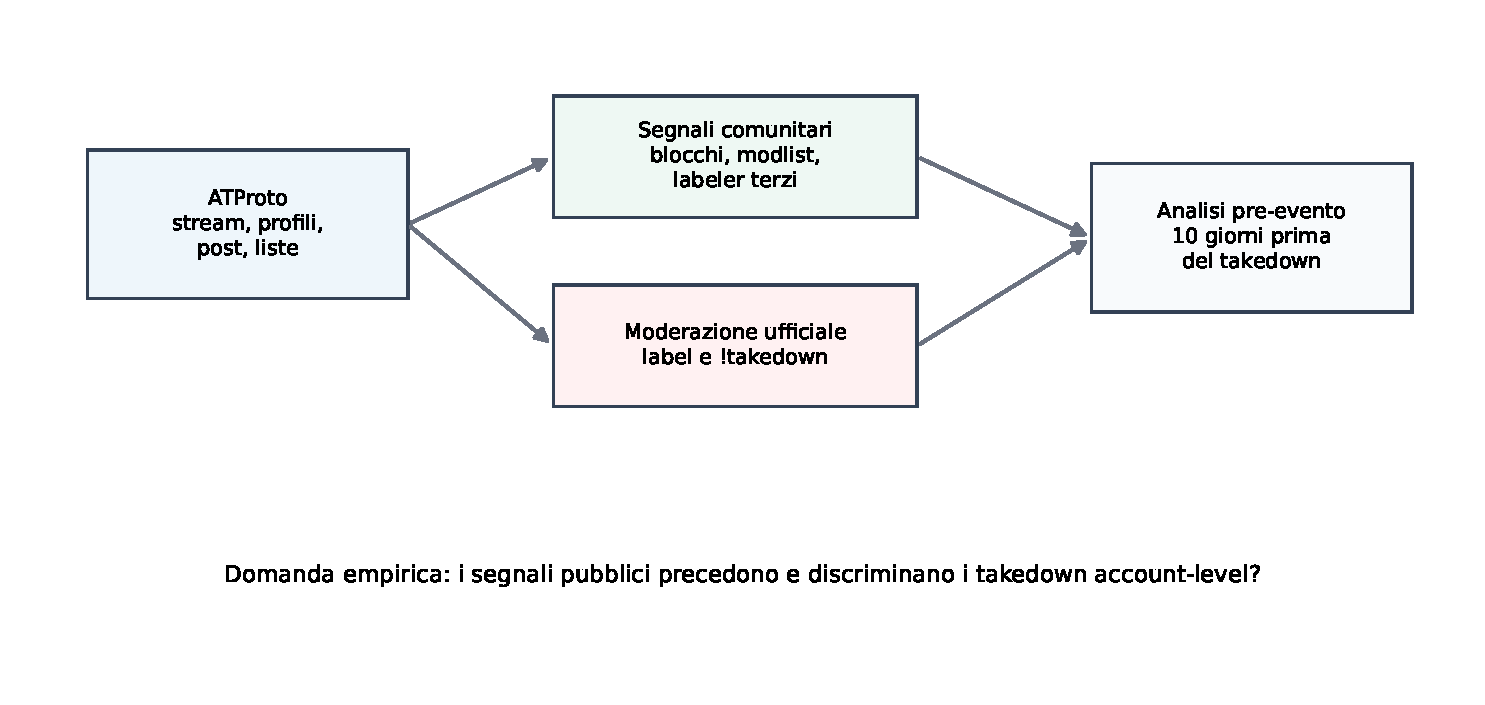
\includegraphics[width=0.95\linewidth]{fig01_architecture.pdf}
  \caption{Architettura concettuale dello studio. I segnali comunitari osservabili vengono misurati nella finestra pre-evento e confrontati con il successivo takedown account-level ufficiale.}
  \label{fig:architecture}
\end{figure}

\section{Stato dell'arte e background}

\subsection{Bluesky e ATProto}

ATProto e' progettato come protocollo componibile per applicazioni sociali. La documentazione ufficiale descrive l'uso di lexicon comuni, repository personali, stream di eventi e servizi applicativi che possono essere implementati da attori diversi \parencite{atprotoOverview, blueskyAtprotoDocs}. A differenza di piattaforme centralizzate tradizionali, Bluesky separa piu' componenti dell'esperienza sociale: archiviazione, indicizzazione, visualizzazione, feed, labels e moderazione. \textcite{balduf2024looking} offrono la prima analisi larga scala della piattaforma, studiandone crescita, attivita' e diversita' dei provider, e rappresentano un riferimento diretto per la struttura dati usata nel presente lavoro.

\subsection{Moderazione componibile}

La documentazione Bluesky descrive la moderazione come un insieme di sistemi sovrapponibili: network takedowns, labels prodotte da servizi di moderazione, e controlli utente come mutes e blocks \parencite{blueskyLabelsModeration}. Questa separazione rende possibile una moderazione piu' pluralistica, nella quale il servizio ufficiale non e' l'unico attore a produrre segnali. La stessa architettura di labeling e' pensata per permettere a servizi indipendenti di pubblicare labels, che poi possono essere interpretate dai client o dagli AppView \parencite{blueskyModerationArchitecture}.

\subsection{Blocchi individuali}

Il blocco individuale e' un'azione pubblica: impedisce interazioni e nasconde l'account bloccato dall'esperienza dell'utente che blocca \parencite{blueskyBlocking}. Questa pubblicita' del record rende i blocchi osservabili come segnale comunitario. In letteratura, \textcite{bono2026selfmoderation} analizzano piu' di 100 milioni di azioni di blocco su Bluesky e mostrano che il blocking puo' essere studiato con profili comportamentali e modelli predittivi. Il presente lavoro usa i blocchi in modo diverso: non predice la propensione a essere bloccati, ma valuta se i blocchi ricevuti prima dell'evento contengano informazione sul successivo takedown ufficiale.

\subsection{Modlist e blocklist}

Le liste utente su Bluesky possono essere curate per feed o usate come modlist. La documentazione definisce \texttt{app.bsky.graph.defs\#modlist} come lista di utenti destinata a muting o blocking \parencite{blueskyUserLists}. Le modlist sono quindi una forma di moderazione comunitaria aggregata: un utente o una comunita' costruisce una lista e altri utenti possono adottarla. \textcite{jhaver2018blocklists} mostrano, nel caso di Twitter, che le blocklist possono proteggere da molestie ma introducono anche problemi di contestazione e accountability. Nel contesto Bluesky, \textcite{sokoto2026open} analizzano individual blocks e blocklists su larga scala, mostrando che le blocklist sono centrali ma eterogenee e concentrate.

\subsection{Labels e labeler indipendenti}

Le labels sono metadati pubblicati da servizi di moderazione; possono applicarsi ad account, record o altri oggetti, e sono interpretate secondo definizioni che determinano se contenuti o account siano nascosti, sfocati, avvertiti o ignorati \parencite{blueskyLabelsModeration}. I labeler indipendenti permettono una moderazione non esclusivamente centralizzata. Questa apertura e' rilevante per il presente lavoro perche' consente di confrontare labels ufficiali, labels di terzi e takedown ufficiali. Tuttavia, come si vedra' nei risultati, il problema empirico principale non e' solo il lift ma la coverage: un segnale molto concentrato nei positivi puo' restare poco utile se compare su una quota minima degli account.

\subsection{Account abusivi, spam e ban evasion}

La moderazione account-level e' spesso legata a problemi di autenticita', spam, impersonation e ban evasion. La letteratura su social bots e account falsi mostra che molte forme di abuso possono essere individuate tramite segnali di attivita', rete e metadati account-level \parencite{ferrara2016rise, varol2017online, cao2012aiding, stringhini2010detecting}. I transparency report di Bluesky collocano questo tema dentro la pratica della piattaforma: nel 2023 vengono menzionati strumenti proattivi contro slurs negli handle e spam accounts, mentre nel 2025 Bluesky descrive un approccio ibrido che combina automazione, sistemi anti-spam e revisione umana \parencite{bluesky2023moderation, bluesky2025transparency}. Queste fonti non identificano la causa dei singoli takedown analizzati qui, ma aiutano a interpretare con prudenza la dinamica del corner 00.

\subsection{Lavori empirici precedenti}

Il progetto si colloca tra tre filoni. Il primo e' lo studio delle architetture decentralizzate e dei protocolli sociali aperti, in cui Bluesky e ATProto sono casi recenti \parencite{balduf2024looking}. Il secondo e' lo studio della moderazione comunitaria e della self-moderation, incluso il ruolo di blocchi, blocklist e strumenti comunitari \parencite{seering2020reconsidering, jhaver2018blocklists, bono2026selfmoderation, sokoto2026open}. Il terzo e' lo studio di enforcement, sospensioni e deplatforming, dove la rimozione o limitazione account-level e' analizzata come decisione di piattaforma con effetti sociali e metodologici non riducibili al singolo contenuto \parencite{gillespie2018custodians, west2018censored, jhaver2021deplatforming}. Rispetto a questi lavori, il presente studio isola una domanda piu' specifica: quanto i segnali pubblici pre-takedown separano account successivamente rimossi da controlli negativi comparabili?

\section{Domande di ricerca}

Le domande di ricerca sono mantenute in numero ridotto e seguono la distinzione tra presenza del segnale, eterogeneita' per esposizione, capacita' predittiva e segnali alternativi.

\begin{description}
  \item[RQ1 -- Presenza e temporalita' del segnale.] Gli account successivamente sottoposti a takedown ricevono piu' blocchi dei controlli comparabili? In quale momento della finestra pre-evento emerge la differenza?
  \item[RQ2 -- Eterogeneita' per esposizione.] Il potere informativo dei blocchi cambia in funzione dell'attivita' e della visibilita' dell'account, con particolare attenzione ai gruppi 00, 0p, p0 e pp?
  \item[RQ3 -- Potere predittivo.] Quanto le feature relative ai blocchi ricevuti consentono a una Random Forest di distinguere gli account positivi dai controlli negativi?
  \item[RQ4 -- Segnali alternativi.] Labels ufficiali, labeler di terze parti e modlist hanno coverage e capacita' discriminante sufficienti per un utilizzo predittivo sistematico?
\end{description}

L'affidabilita' della label \code{!takedown} e' trattata come controllo preliminare sulla validita' del target. Non e' formulata come domanda autonoma perche' serve soprattutto a stabilire se il target operativo sia abbastanza stabile da supportare l'analisi successiva.

\section{Parte sperimentale: dati e metodi}

\subsection{Origine e struttura dei dati}

L'analisi usa dataset concessi dal gruppo di ricerca guidato da Balduf e dataset derivati costruiti nel progetto a partire da dati osservabili tramite ATProto. Le fonti operative includono profili, post, blocchi, liste, elementi delle liste, adozione delle liste, labels ufficiali e labels prodotte da labeler indipendenti. I dati riguardano principalmente marzo 2026 e sono arricchiti con log del labeler ufficiale.

Per ragioni di minimizzazione del dato, i dati grezzi non anonimizzati sono rimasti sulla macchina virtuale di analisi. Localmente sono stati usati dataset derivati e anonimizzati: i DID reali sono stati sostituiti da identificativi anonimi e i dataset impiegati nel report contengono variabili aggregate, metadati temporali e indicatori di segnale, non contenuti testuali personali.

La scala dei dati e' riassunta in \cref{tab:scale}. La manifest associata a marzo include \num{4189} file di log; alcuni file possono contenere eventi con timestamp appartenenti anche ad altri mesi. Per questo i conteggi sui takedown sono sempre basati sul filtro temporale dell'evento, non sulla sola appartenenza del file alla manifest.

\begin{table}[htbp]
  \centering
  \caption{Scala dei dataset principali usati nello studio.}
  \label{tab:scale}
  \begin{tabularx}{\linewidth}{X r}
    \toprule
    Quantita' & Valore \\
    \midrule
    DID distinti nei profili & \num{1222452} \\
    File di log nella manifest di marzo & \num{4189} \\
    Righe post nel periodo operativo & \num{36946883} \\
    Eventi account-level \code{!takedown} non-neg in marzo & \num{159161} \\
    Account positivi unici in marzo & \num{158803} \\
    Positivi nel dataset operativo 11--21 marzo & \num{47821} \\
    Account negativi distinti & \num{366515} \\
    Osservazioni negative account-giorno & \num{4031665} \\
    \bottomrule
  \end{tabularx}
\end{table}

\subsection{Software e ambiente di analisi}

Le elaborazioni sono state svolte in Python, con DuckDB per interrogare file Parquet e CSV compressi, pandas e NumPy per la manipolazione tabellare, scikit-learn per la Random Forest e LaTeX per la redazione del report. DuckDB e' stato usato perche' permette query SQL su file colonnari di grandi dimensioni senza caricarli integralmente in memoria, mantenendo riproducibili le aggregazioni su blocchi, post e labels.

\subsection{Definizione del target}

Il target positivo e' un evento account-level \code{!takedown} non-neg emesso dal servizio ufficiale. Gli eventi con \code{neg=true} sono trattati come revoche. Per ogni account positivo si usa il primo takedown osservabile come \code{event_time}. In marzo sono stati osservati \num{159161} eventi non-neg su \num{158803} account positivi unici. Le revoche sono \num{3705}, pari al \pct{2,2749} degli eventi totali \code{!takedown}; gli account positivi con revoca successiva sono \num{2814}, pari al \pct{1,772} dei positivi. Gli account con piu' di un takedown non-neg sono \num{325}, circa lo \pct{0,20}; la distanza media tra primo e secondo takedown e' circa \num{31.8} ore, mentre la distanza media tra primo takedown e prima revoca e' circa \num{44.4} ore.

Questi valori indicano che \code{!takedown} e' un proxy operativo abbastanza stabile per l'enforcement account-level, pur con eccezioni non trascurabili. Per questo la validita' del target e' trattata come controllo preliminare, non come risultato causale.

\subsection{Utility window}

Per ogni account $i$ viene definita una finestra pre-evento:
\[
W_i=[T_i-10\text{ giorni},T_i),
\]
dove $T_i$ e' il primo takedown per i positivi e uno pseudo-event time per i negativi. Il timestamp esatto $T_i$ e' escluso dalla finestra.

La utility window e' stimata con una procedura positive-only: per ciascun account positivo si identifica il primo takedown osservabile, si considerano i post precedenti all'evento, si calcola la distanza temporale tra post e takedown, si stima il quantile $q80_i$ per account e infine si calcola $Q_{75}(q80_i)$ sugli account con storia sufficiente. La finestra operativa viene scelta come la piu' piccola finestra della griglia candidata superiore alla soglia. Il risultato adottato nelle analisi successive e' una utility window di dieci giorni. \Cref{fig:utility} visualizza la definizione temporale.

\begin{figure}[htbp]
  \centering
  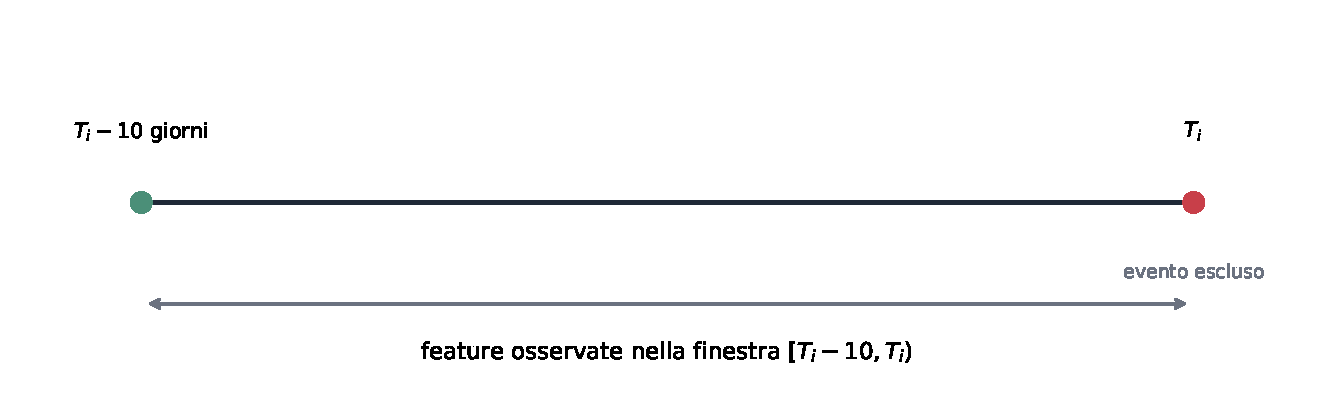
\includegraphics[width=0.86\linewidth]{fig02_utility_window.pdf}
  \caption{Utility window di dieci giorni. Le feature sono calcolate nell'intervallo $[T_i-10,T_i)$; il timestamp dell'evento e' escluso.}
  \label{fig:utility}
\end{figure}

\subsection{Costruzione dei positivi e dei negativi}

I positivi sono account con almeno un evento \code{!takedown} non-neg. Tre denominatori devono restare distinti: nel bucket 11--20 marzo si osservano \num{44395} account positivi distinti e \num{44462} eventi; il dataset operativo usato per le analisi pre-evento comprende invece \num{47821} positivi nei giorni 11--21 marzo inclusi. I valori non sono sinonimi.

I negativi sono account osservabili a marzo, creati prima dell'inizio del mese e privi di takedown nel periodo osservato. A ciascun negativo viene assegnato uno pseudo-event time negli stessi giorni dei positivi. Questa assegnazione riduce il confondimento dovuto al calendario, ma non dimostra da sola l'assenza di takedown successivi oltre la finestra osservata. La pipeline metodologica complessiva e' sintetizzata in \cref{fig:pipeline}.

\begin{figure}[htbp]
  \centering
  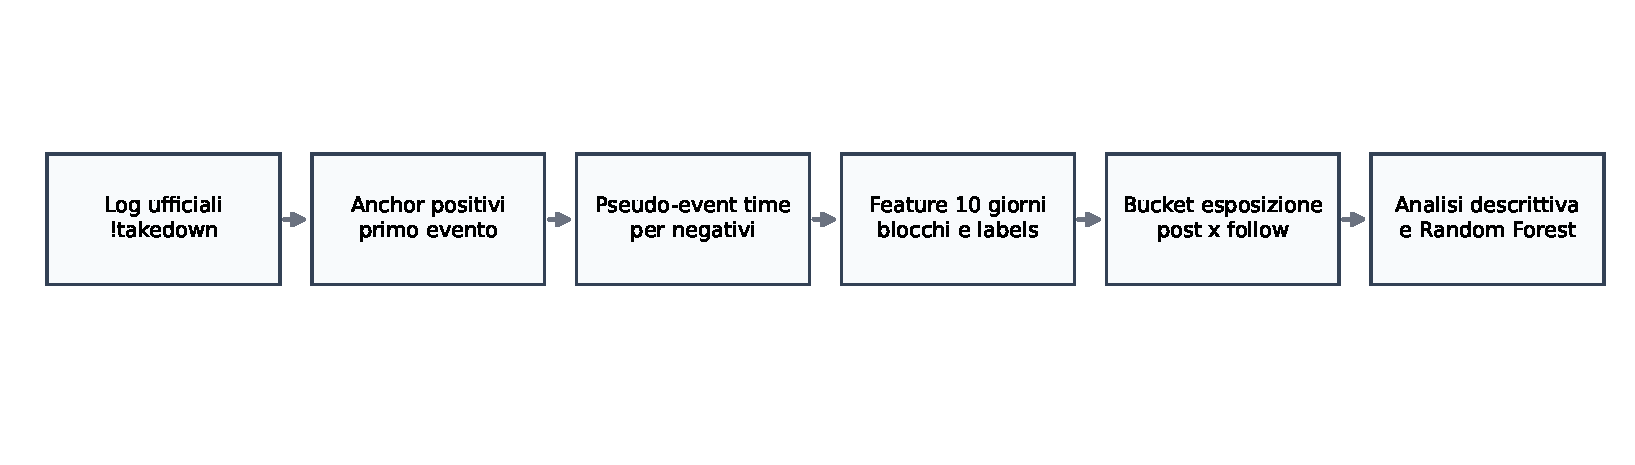
\includegraphics[width=0.95\linewidth]{fig03_pipeline.pdf}
  \caption{Pipeline metodologica: costruzione del target, assegnazione degli pseudo-event time, calcolo dei segnali pre-evento, controllo per esposizione e analisi predittiva.}
  \label{fig:pipeline}
\end{figure}

\subsection{Variabili di esposizione e bucket}

Il numero di blocchi ricevuti dipende dall'esposizione pubblica dell'account. Per questo l'analisi controlla due dimensioni: attivita', misurata tramite \code{n_posts_10d}, e visibilita', misurata tramite \code{incoming_follows_10d}. I bucket lineari usati sono: 0, 1, 2, 3--5, 6--10, 11--25, 26--50, 51--100, 101--250, 251--500, 501--1000 e 1001+. L'indice congiunto e' definito come
\[
b_{pf}=100\cdot b_p+b_f,
\]
con $b_p$ pari al bucket dei post e $b_f$ pari al bucket dei follow ricevuti. La scelta di bucket lineari, anziche' quantili, privilegia interpretabilita' e somiglianza sostanziale tra account. I quattro corner sono: 00, zero post e zero follow ricevuti; 0p, zero post e almeno un follow; p0, almeno un post e zero follow; pp, almeno un post e almeno un follow.

\subsection{Segnali analizzati}

I segnali principali sono il numero totale di blocchi ricevuti, il numero di blocker unici, la distribuzione giornaliera dei blocchi, la presenza in modlist, le labels ufficiali post-level e account-level, e le labels prodotte da labeler terzi. Per ciascun segnale si distinguono presenza, intensita', temporalita', coverage e lift. Il lift e' definito come
\[
\operatorname{Lift}=\frac{P(S=1\mid Y=1)}{P(S=1\mid Y=0)}.
\]
Un lift alto non implica automaticamente utilita' predittiva se la coverage e' molto bassa.

\subsection{Random Forest e validazione}

La Random Forest e' usata come modello predittivo non causale. L'analisi principale usa il pool massimo con corner 00 escluso, gruppi 0p, p0 e pp bilanciati, \num{28650} osservazioni complessive, \num{14325} positivi e \num{14325} negativi. La validazione riportata usa predizioni out-of-fold su un campione stratificato di training pari al 70\% del dataset bilanciato, con \code{StratifiedKFold} a 10 fold.

Il modello usa \num{1000} alberi, foglia minima pari a 5, profondita' non vincolata, nessun class weighting e random state 42. La specificazione principale include 11 feature: \code{n_unique_blockers_10d} e le dieci variabili giornaliere da \code{day_0} a \code{day_9}. L'interpretazione del modello usa la Random Forest feature importance basata sulla riduzione dell'impurita'.

\section{Risultati}

\subsection{Distribuzione per corner}

La distribuzione per corner mostra una composizione molto diversa tra positivi e negativi (\cref{tab:corner,fig:corner}). Il corner 00 rappresenta il \pct{60,23} dei positivi e il \pct{33,81} dei negativi. Gli account pp, cioe' con almeno un post e almeno un follow ricevuto, sono invece il \pct{38,55} dei negativi e il \pct{17,42} dei positivi.

\begin{table}[!htbp]
  \centering
  \caption{Distribuzione degli account per corner di esposizione. Percentuali calcolate su account distinti per campione.}
  \label{tab:corner}
  \begin{tabular}{lrr}
    \toprule
    Corner & Negativi & Positivi \\
    \midrule
    00 & \pct{33,81} & \pct{60,23} \\
    0p & \pct{10,43} & \pct{12,37} \\
    p0 & \pct{17,21} & \pct{9,99} \\
    pp & \pct{38,55} & \pct{17,42} \\
    \bottomrule
  \end{tabular}
\end{table}

\begin{figure}[!htbp]
  \centering
  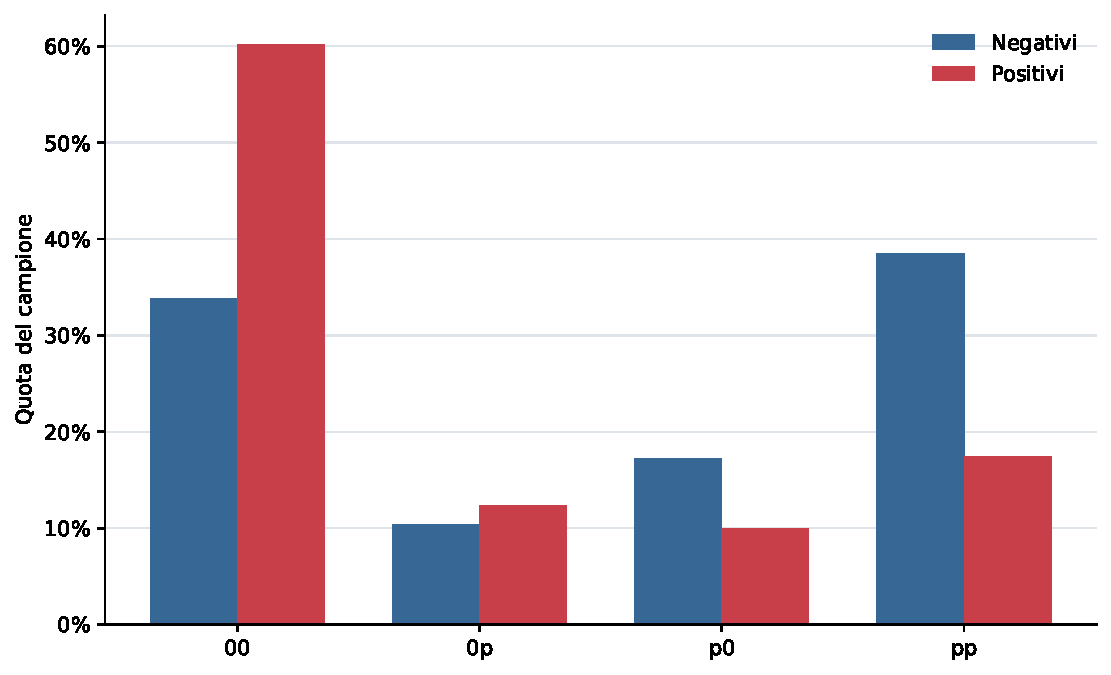
\includegraphics[width=0.8\linewidth]{fig04_corner_distribution.pdf}
  \caption{Distribuzione per corner di esposizione. Il corner 00 e' sovrarappresentato tra i positivi.}
  \label{fig:corner}
\end{figure}

\FloatBarrier
\subsection{Corner 00}

Il corner 00 richiede due statistiche distinte. Sul campione completo dei positivi con \code{created_at} disponibile ($N=\num{20205}$), la lifetime media e' \num{1.7476} giorni, circa 42 ore, mentre la mediana e' \num{0.000081} giorni. Nel sottoinsieme degli account 00 con lifetime inferiore a dieci giorni, su \num{20574} account 00 totali considerati, \num{19530} rientrano nella condizione, pari al \pct{94,9}; la media condizionata e' \num{0.378466} giorni, circa \num{9.1} ore. Non si tratta quindi di una singola media generale di nove ore, ma di una media condizionata.

\Cref{fig:lifetime} confronta la lifetime per corner tra i positivi con \code{created_at} disponibile. Nel dataset dedicato ai blocchi, anche i 00 positivi ricevono piu' blocchi dei 00 negativi, ma i livelli assoluti restano bassi (\cref{tab:corner00blocks}).

\begin{figure}[!htbp]
  \centering
  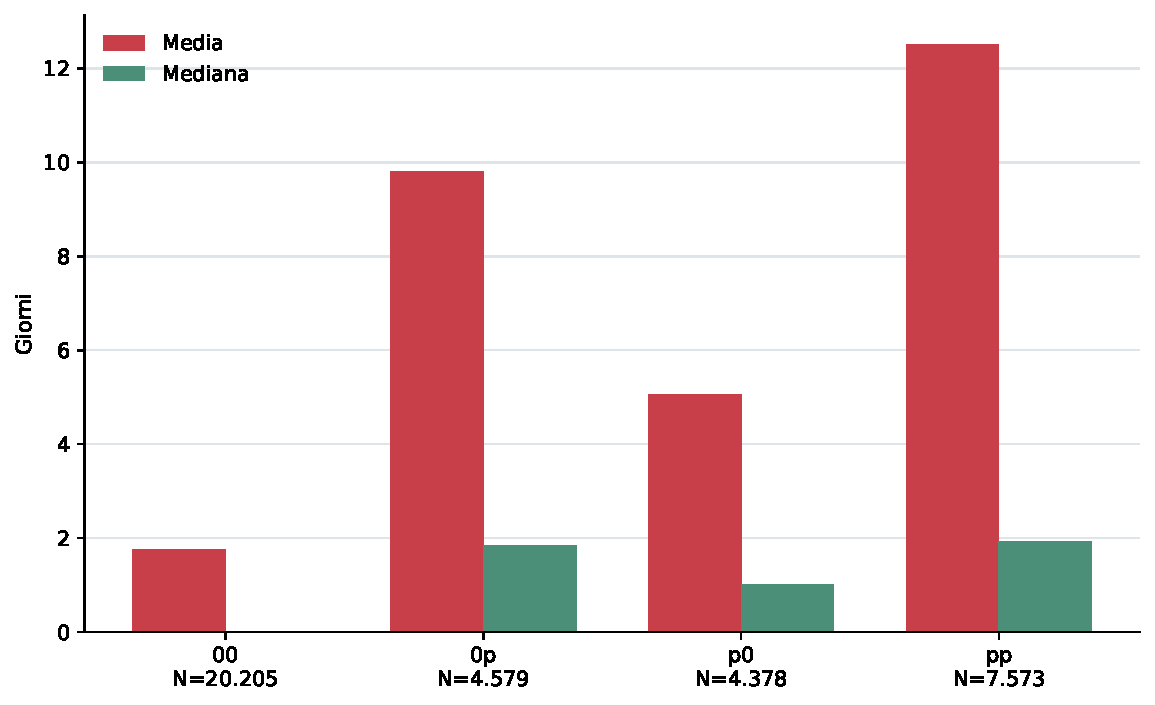
\includegraphics[width=0.82\linewidth]{fig05_lifetime_corner.pdf}
  \caption{Lifetime media e mediana dei positivi per corner, sugli account con \code{created_at} disponibile.}
  \label{fig:lifetime}
\end{figure}

\begin{table}[!htbp]
  \centering
  \caption{Blocchi nel corner 00. Le mediane dei blocchi sono zero in entrambi i gruppi.}
  \label{tab:corner00blocks}
  \scriptsize
  \setlength{\tabcolsep}{2.8pt}
  \begin{tabular}{lrrrr}
    \toprule
    Campione & Obs. 00 & Rate & Blocchi & Uniq. blockers \\
    \midrule
    Negativi & \num{1341731} & \pct{1,40} & \num{0.0175} & \num{0.0168} \\
    Positivi & \num{28802} & \pct{3,71} & \num{0.0867} & \num{0.0861} \\
    \bottomrule
  \end{tabular}
\end{table}

\FloatBarrier
\subsection{Confronto generale dei blocchi}

Nel confronto generale i positivi ricevono piu' frequentemente almeno un blocco nei dieci giorni pre-evento e accumulano piu' blocchi in media (\cref{tab:blocks-general,fig:blocks-general}). Il \pct{27,82} dei positivi ha almeno un blocco, contro il \pct{18,09} dei negativi; i blocchi medi sono \num{3.2787} per i positivi e \num{1.1073} per i negativi.

\begin{table}[!htbp]
  \centering
  \caption{Statistiche generali sui blocchi ricevuti nella finestra di dieci giorni.}
  \label{tab:blocks-general}
  \begin{tabularx}{\linewidth}{Xrr}
    \toprule
    Indicatore & Negativi & Positivi \\
    \midrule
    Osservazioni & \num{4031665} & \num{47821} \\
    Account distinti & \num{366515} & \num{47821} \\
    Almeno un blocco nei 10 giorni & \pct{18,09} & \pct{27,82} \\
    Blocchi medi & \num{1.1073} & \num{3.2787} \\
    P95 blocchi & \num{3} & \num{9} \\
    Unique blockers medi & \num{1.0873} & \num{3.2485} \\
    \bottomrule
  \end{tabularx}
\end{table}

\begin{figure}[!htbp]
  \centering
  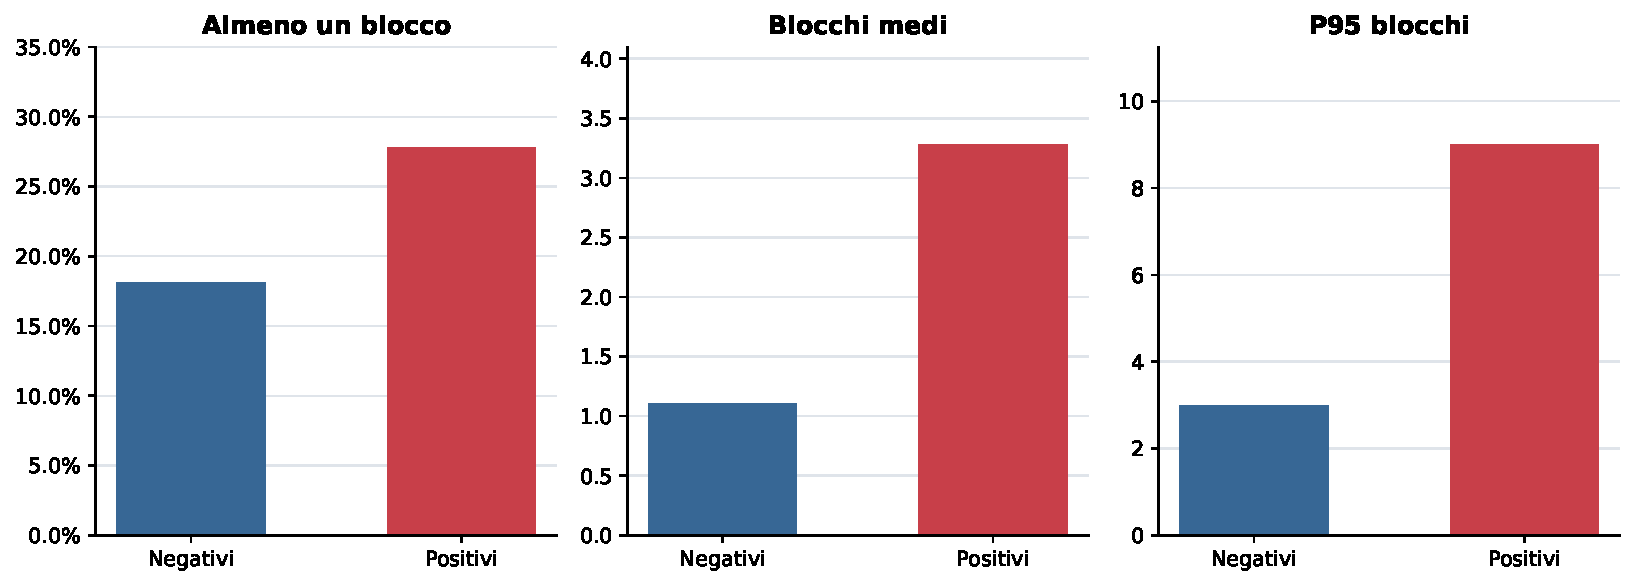
\includegraphics[width=0.88\linewidth]{fig06_blocks_general.pdf}
  \caption{Confronto generale dei blocchi ricevuti: presenza di almeno un blocco, blocchi medi e P95.}
  \label{fig:blocks-general}
\end{figure}

\FloatBarrier
\subsection{Controllo per esposizione}

Il controllo per post bucket mostra che nei bucket bassi i positivi hanno generalmente una probabilita' piu' elevata di ricevere almeno un blocco e accumulano piu' blocchi medi. Nei bucket molto esposti anche i negativi possono ricevere blocchi frequentemente, ma l'intensita' media dei positivi resta spesso piu' alta (\cref{fig:post-bucket}). La matrice post $\times$ follow in \cref{fig:heatmap} conferma che il rapporto tra positivi e negativi deve essere letto entro celle di esposizione comparabili e con supporto sufficiente.

\begin{figure}[!htbp]
  \centering
  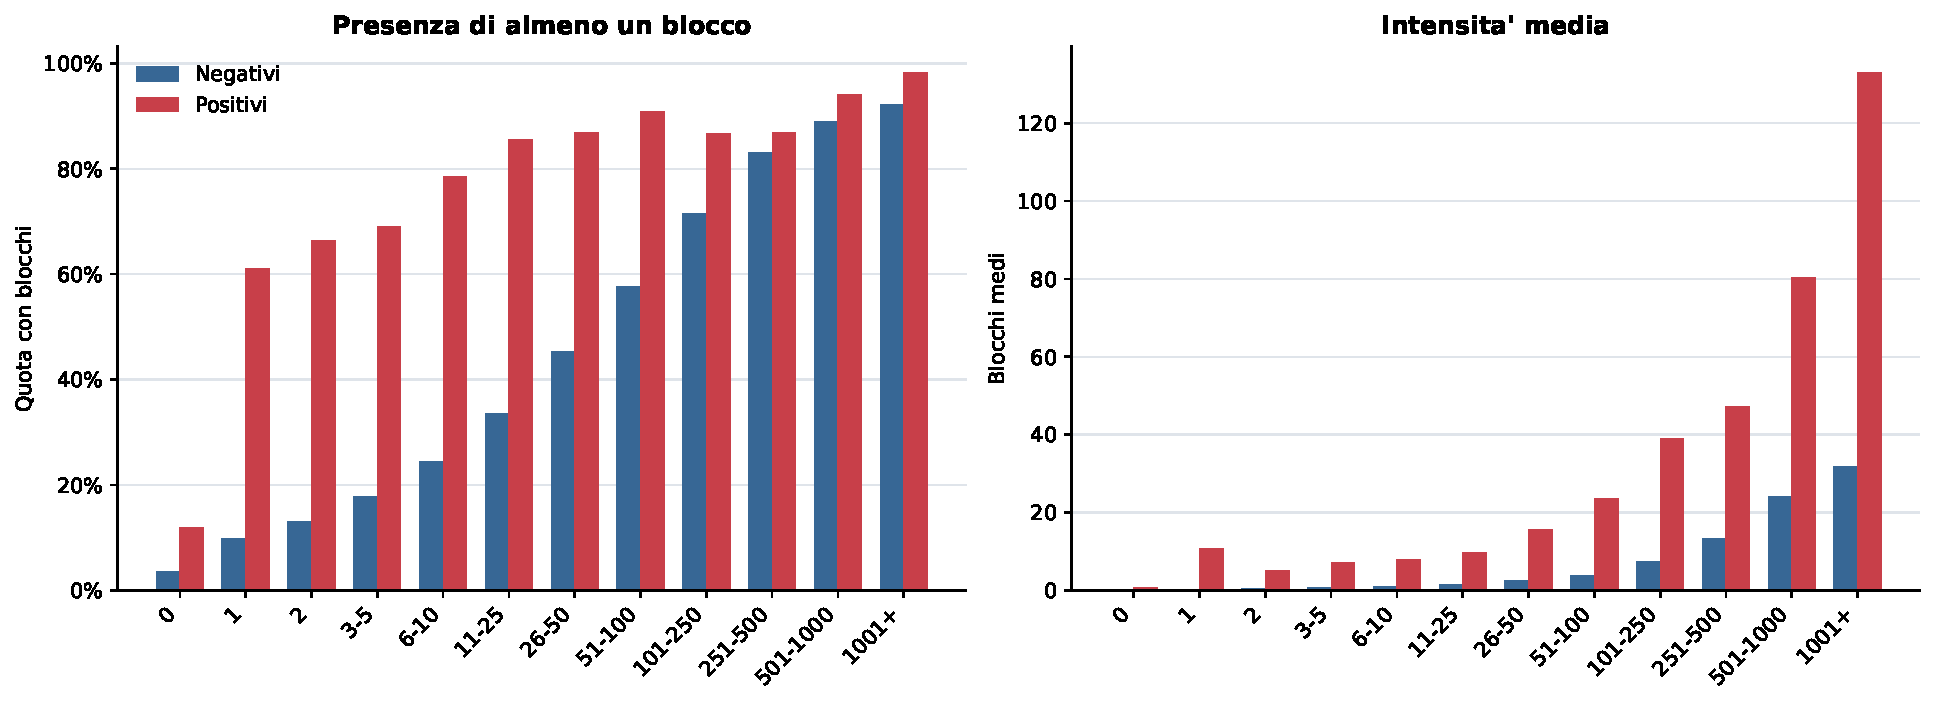
\includegraphics[width=\linewidth]{fig07_post_bucket_blocks.pdf}
  \caption{Blocchi per post bucket. A sinistra quota con almeno un blocco; a destra blocchi medi nei dieci giorni pre-evento.}
  \label{fig:post-bucket}
\end{figure}

\begin{figure}[!htbp]
  \centering
  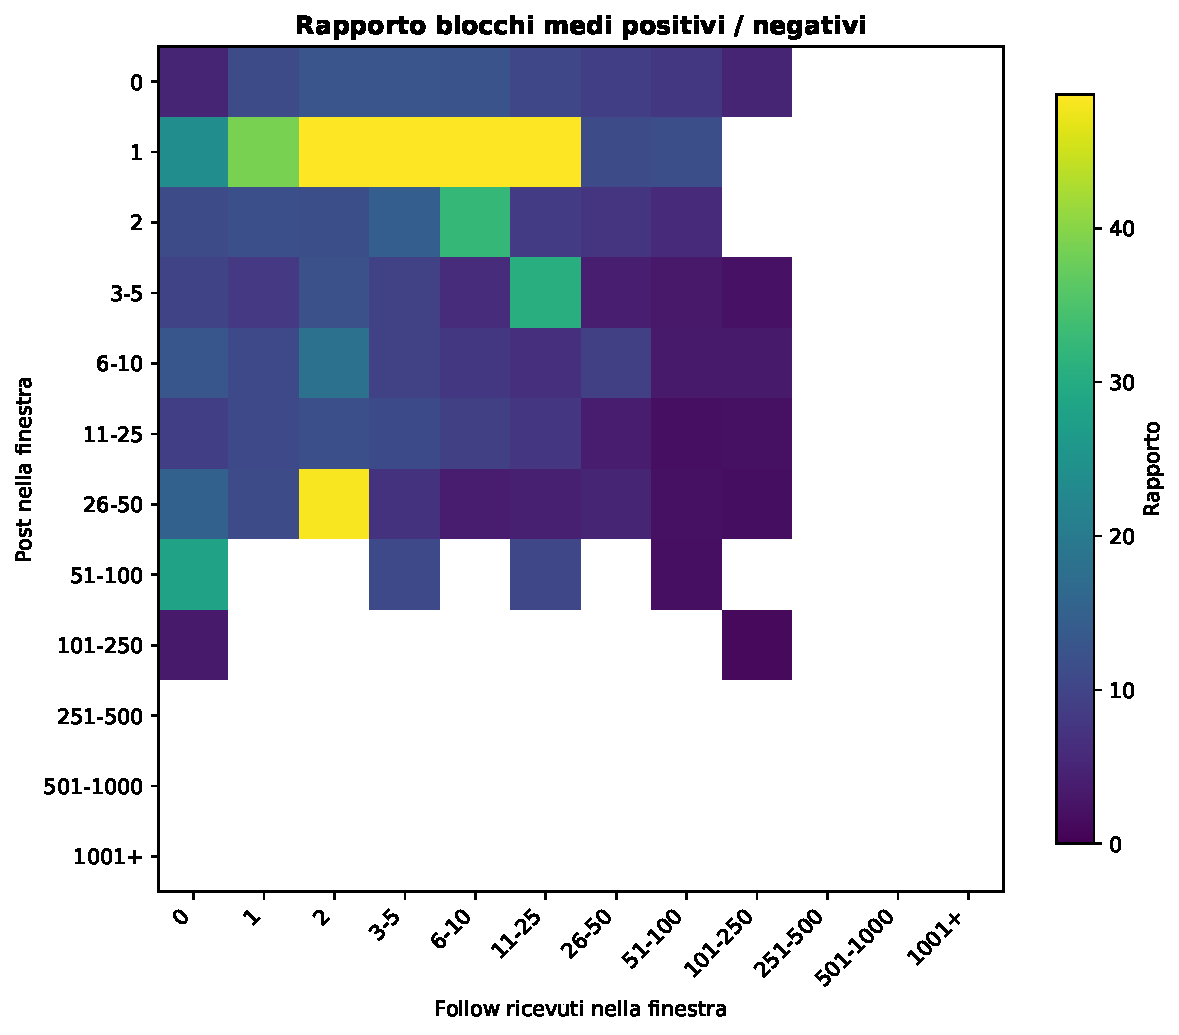
\includegraphics[width=0.82\linewidth]{fig08_exposure_heatmap.pdf}
  \caption{Heatmap del rapporto tra blocchi medi dei positivi e dei negativi per bucket congiunti post $\times$ follow. Le celle con supporto insufficiente sono mascherate.}
  \label{fig:heatmap}
\end{figure}

\FloatBarrier
\subsection{Temporalita' del segnale}

Escludendo il corner 00, i blocchi dei positivi sono fortemente concentrati vicino all'evento. Il \pct{55,63} dei blocchi dei positivi cade nell'ultimo giorno pre-evento, contro il \pct{10,75} dei negativi; negli ultimi tre giorni la quota sale al \pct{78,77} per i positivi e al \pct{31,10} per i negativi (\cref{tab:timing,fig:timing}). Nella notazione delle feature, \code{day_0} indica il giorno immediatamente precedente all'evento; nel grafico e' visualizzato come giorno $-1$. Il timestamp esatto del takedown non entra nelle feature.

\begin{table}[!htbp]
  \centering
  \caption{Distribuzione temporale dei blocchi, corner 00 escluso. Percentuali condizionate agli account con almeno un blocco.}
  \label{tab:timing}
  \scriptsize
  \setlength{\tabcolsep}{3pt}
  \begin{tabular}{lrrr}
    \toprule
    Campione & Ultimo giorno & Ultimi 3 giorni & Giorni prec. \\
    \midrule
    Negativi & \pct{10,75} & \pct{31,10} & \pct{68,90} \\
    Positivi & \pct{55,63} & \pct{78,77} & \pct{21,23} \\
    \bottomrule
  \end{tabular}
\end{table}

\begin{figure}[!htbp]
  \centering
  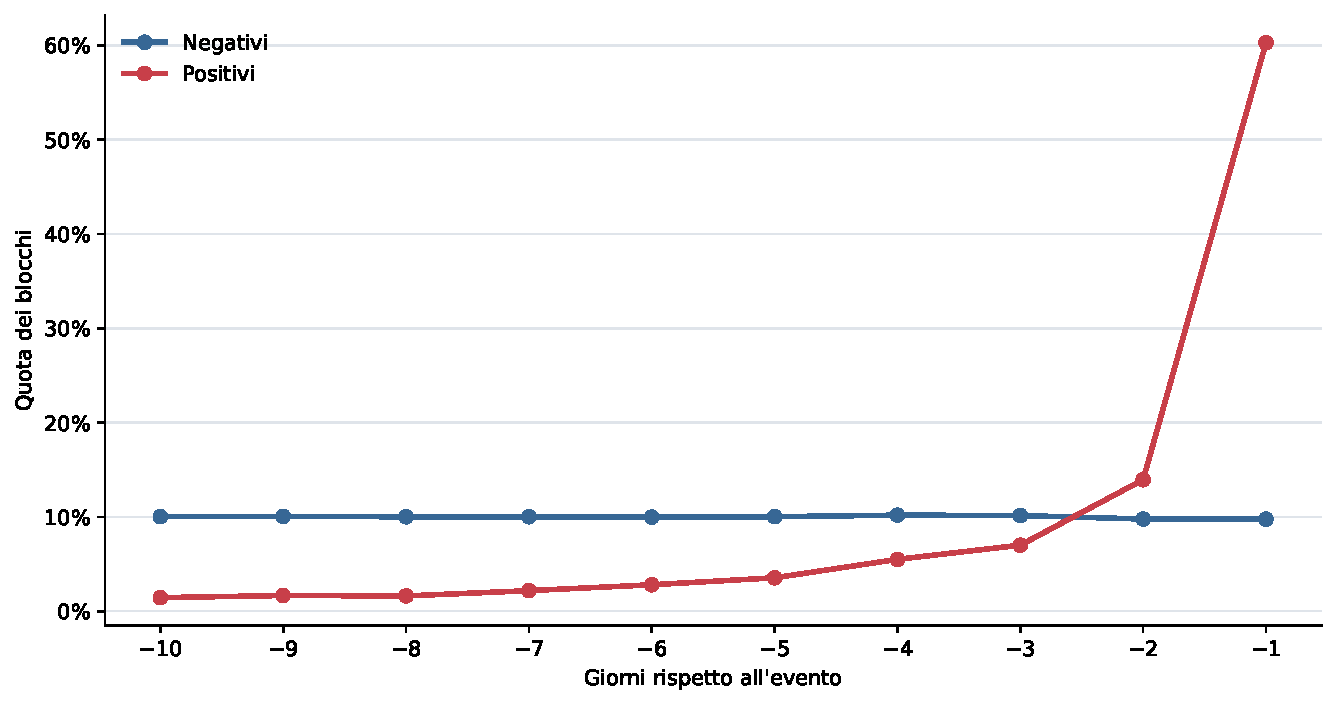
\includegraphics[width=\linewidth]{fig09_daily_timing.pdf}
  \caption{Distribuzione giornaliera dei blocchi nella finestra pre-evento, corner 00 escluso.}
  \label{fig:timing}
\end{figure}

\FloatBarrier
\subsection{Progressione Random Forest}

La performance predittiva cambia sensibilmente con la costruzione del campione (\cref{tab:rf-progress,fig:rf-progress}). Il setup con F1 pari a \num{0.728} non e' direttamente comparabile all'analisi principale, perche' esclude sia il corner 00 sia bucket adiacenti e usa un criterio di campionamento diverso. L'analisi principale e' il setup 6, con pool massimo, tre gruppi esposti bilanciati e 11 feature.

\begin{table}[!htbp]
  \centering
  \caption{Progressione degli esperimenti Random Forest. I valori riportano F1 out-of-fold in cross-validation.}
  \label{tab:rf-progress}
  \scriptsize
  \setlength{\tabcolsep}{2.5pt}
  \begin{tabularx}{\linewidth}{rXlrr}
    \toprule
    Setup & Campione & Corner & Feat. & CV F1 \\
    \midrule
    1 & ca. 1.000+1.000 & 00 incluso & 28 & \num{0.371} \\
    2 & ca. 1.000+1.000 & 00 incluso & 11 & \num{0.382} \\
    3 & ca. 10.000+10.000 & 00 incluso & 11 & \num{0.377} \\
    4 & ca. 10.000+10.000 & no 00/adiacenti & 11 & \num{0.728} \\
    5 & 4 gruppi bilanciati & 00 incluso & 11 & \num{0.563} \\
    6 & 28.650, 3 gruppi & 00 escluso & 11 & \num{0.688} \\
    \bottomrule
  \end{tabularx}
\end{table}

\begin{figure}[!htbp]
  \centering
  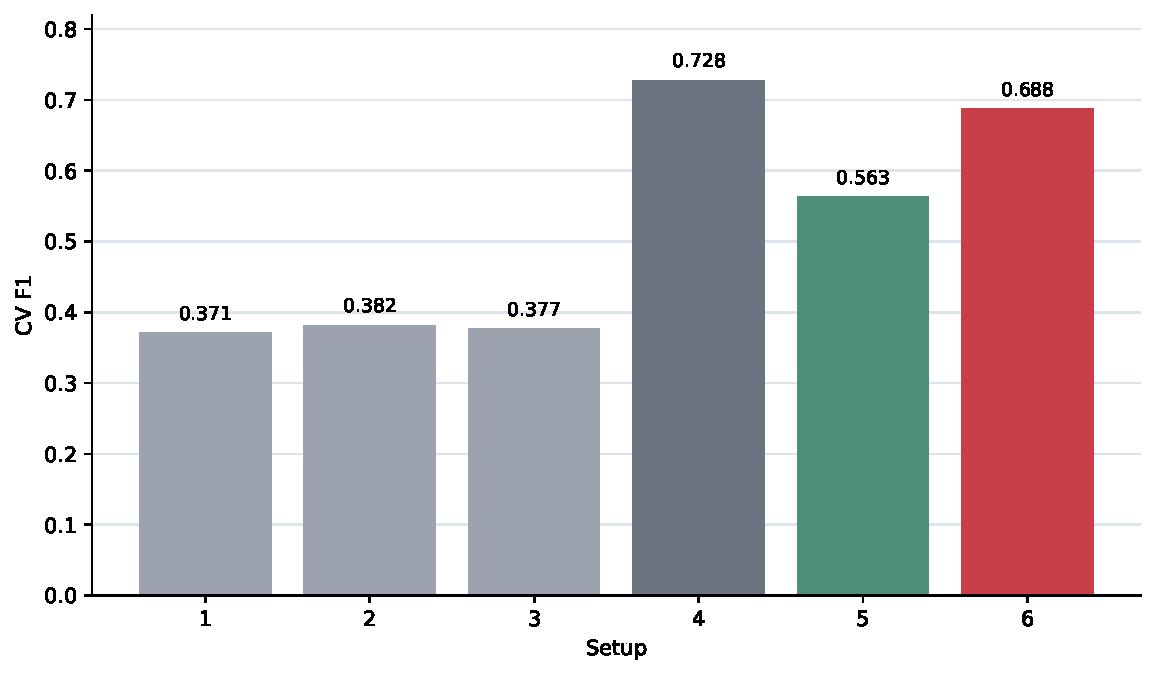
\includegraphics[width=0.86\linewidth]{fig10_rf_progression.pdf}
  \caption{F1 cross-validato nei sei setup Random Forest. Le differenze riflettono anche scelte di campionamento e inclusione dei corner.}
  \label{fig:rf-progress}
\end{figure}

\FloatBarrier
\subsection{Analisi principale}

Nel setup principale la Random Forest raggiunge sul training CV F1 medio \num{0.6876} con deviazione standard \num{0.0134}. Le predizioni out-of-fold sul training producono accuracy \num{0.7385}, precision \num{0.8534}, recall \num{0.5760}, F1 \num{0.6878} e ROC AUC \num{0.7604}. La matrice di confusione cross-validata sul training e':
\[
\begin{pmatrix}
9035 & 992\\
4252 & 5776
\end{pmatrix}.
\]

Dopo il fit finale su tutto il training set, la valutazione held-out sul test set produce accuracy \num{0.7268}, precision \num{0.8409}, recall \num{0.5595}, F1 \num{0.6719} e ROC AUC \num{0.7535}. La matrice di confusione sul test set e':
\[
\begin{pmatrix}
3843 & 455\\
1893 & 2404
\end{pmatrix}.
\]

Il controllo sui DID anonimizzati non mostra sovrapposizioni: \num{0} DID in comune tra training e test e nessun DID condiviso tra fit e validation fold nella cross-validation stratificata.

\FloatBarrier
\subsection{Risultati per corner esposto}

La performance varia tra gruppi esposti (\cref{tab:corner-rf,fig:corner-rf}). Sul test held-out il gruppo pp e' il piu' classificabile, con ROC AUC \num{0.821} e F1 per i positivi \num{0.745}; 0p e p0 mostrano precision elevata ma recall piu' bassa. I valori cross-validati sul training restano coerenti e leggermente superiori per F1 globale.

\begin{table}[!htbp]
  \centering
  \caption{Metriche per macro-gruppo, predizioni out-of-fold.}
  \label{tab:corner-rf}
  \scriptsize
  \setlength{\tabcolsep}{2.5pt}
  \begin{tabular}{lrrrrrr}
    \toprule
    Gruppo & $N$ & Acc. & ROC AUC & F1 pos. & Prec. pos. & Recall pos. \\
    \midrule
    0p & \num{6656} & \num{0.721} & \num{0.726} & \num{0.630} & \num{0.923} & \num{0.479} \\
    p0 & \num{6768} & \num{0.738} & \num{0.748} & \num{0.660} & \num{0.927} & \num{0.512} \\
    pp & \num{6631} & \num{0.757} & \num{0.819} & \num{0.754} & \num{0.773} & \num{0.736} \\
    \bottomrule
  \end{tabular}
\end{table}

\begin{figure}[!htbp]
  \centering
  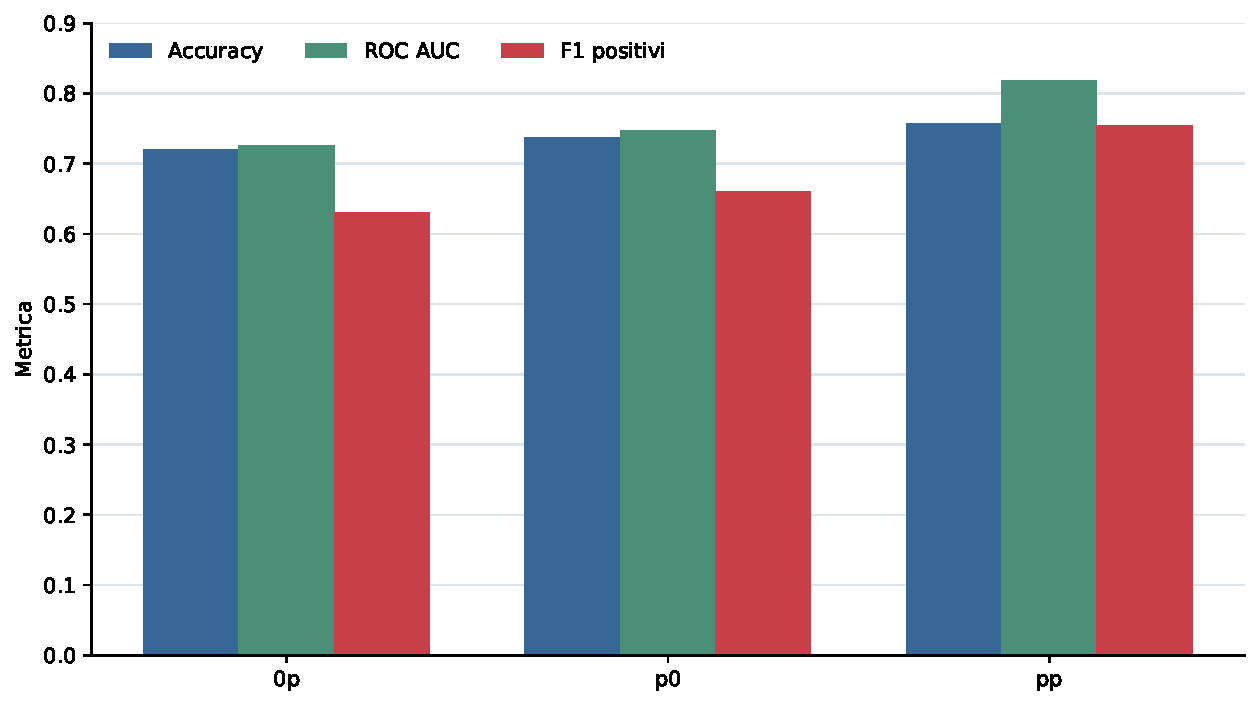
\includegraphics[width=0.86\linewidth]{fig11_corner_performance.pdf}
  \caption{Performance held-out del modello principale per corner esposto.}
  \label{fig:corner-rf}
\end{figure}

\FloatBarrier
\subsection{Feature importance}

L'interpretazione usa l'impurity-based feature importance nativa della Random Forest. Nelle analisi a 11 feature, \code{n_unique_blockers_day_0} emerge stabilmente come la variabile piu' importante; nel setup bilanciato sui quattro corner la sua importanza e' \num{0.4424}, seguita da \code{n_unique_blockers_10d} con \num{0.2778} e \code{n_unique_blockers_day_1} con \num{0.0664} (\cref{fig:feature-importance}). Questi valori sono presentati come indicazione interpretativa del peso relativo dei segnali giornalieri, non come stima causale: la misura non indica il segno dell'effetto e puo' essere influenzata dalla correlazione tra feature.

\begin{figure}[!htbp]
  \centering
  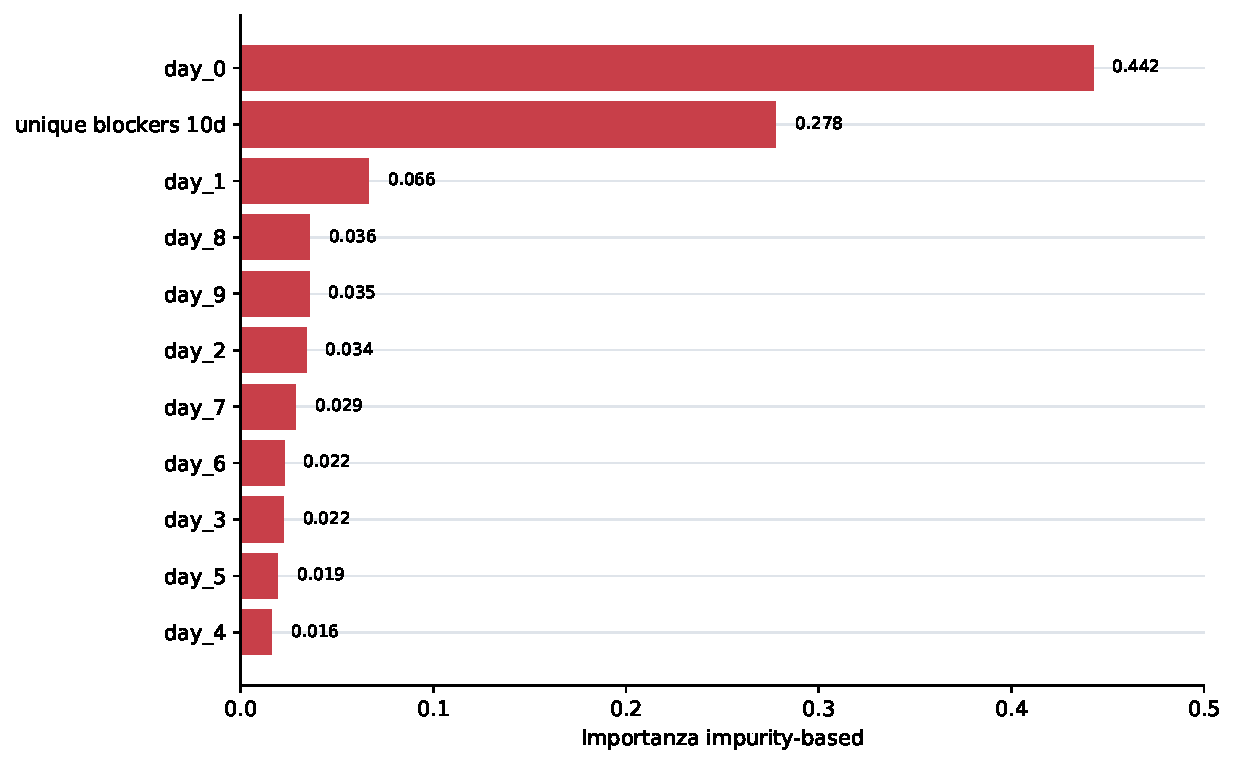
\includegraphics[width=0.86\linewidth]{fig12_feature_importance.pdf}
  \caption{Random Forest feature importance nel setup a 11 feature bilanciato sui quattro corner.}
  \label{fig:feature-importance}
\end{figure}

\FloatBarrier
\subsection{Labels e modlist}

Le labels ufficiali post-level coprono una quota limitata dei positivi: su \num{47821} positivi, \num{1121} hanno almeno una label post-level nei dieci giorni pre-takedown, pari al \pct{2,344}. Le labels piu' frequenti sono \code{sexual}, con \num{761} positivi (\pct{1,591}), e \code{porn}, con \num{499} positivi (\pct{1,043}). Queste labels vanno distinte dalle labels ufficiali account-level e dal target \code{!takedown}.

I labeler di terze parti mostrano talvolta lift elevati ma coverage bassa (\cref{tab:third-labelers}). L'analisi dei negativi per alcuni labeler e' stata condotta su campioni disponibili, non necessariamente sull'intera popolazione negativa; il campione negativo documentato raggiunge \num{37566} account quando disponibile.

\begin{table}[!htbp]
  \centering
  \caption{Coverage e lift dei labeler di terze parti.}
  \label{tab:third-labelers}
  \scriptsize
  \setlength{\tabcolsep}{2.8pt}
  \begin{tabular}{llrrr}
    \toprule
    Labeler & Livello & Positivi & Negativi & Lift \\
    \midrule
    Skywatch Blue & Account & \pct{2,944} & \pct{0,695} & \num{4.24} \\
    Blacksky Moderation & Account & \pct{0,090} & \pct{0,006} & \num{14.27} \\
    Profile Labeller & Account & \pct{1,913} & \pct{0,155} & \num{12.36} \\
    Skywatch Blue & Post & \pct{1,094} & \pct{1,209} & \num{0.90} \\
    Blacksky Moderation & Post & \pct{0,004} & \pct{0,008} & \num{0.50} \\
    \bottomrule
  \end{tabular}
\end{table}

Le modlist hanno coverage ancora piu' bassa: su \num{47821} positivi, \num{929} sono inclusi in almeno una modlist nei dieci giorni precedenti, pari al \pct{1,943}. Le relazioni account--modlist osservate sono \num{1033}, distribuite su \num{73} modlist distinte; tra i soli positivi inclusi, la media e' \num{1.09}, la mediana e' 1 e il massimo e' 7. \Cref{fig:coverage-lift} confronta coverage e lift dei segnali alternativi.

\begin{figure}[!htbp]
  \centering
  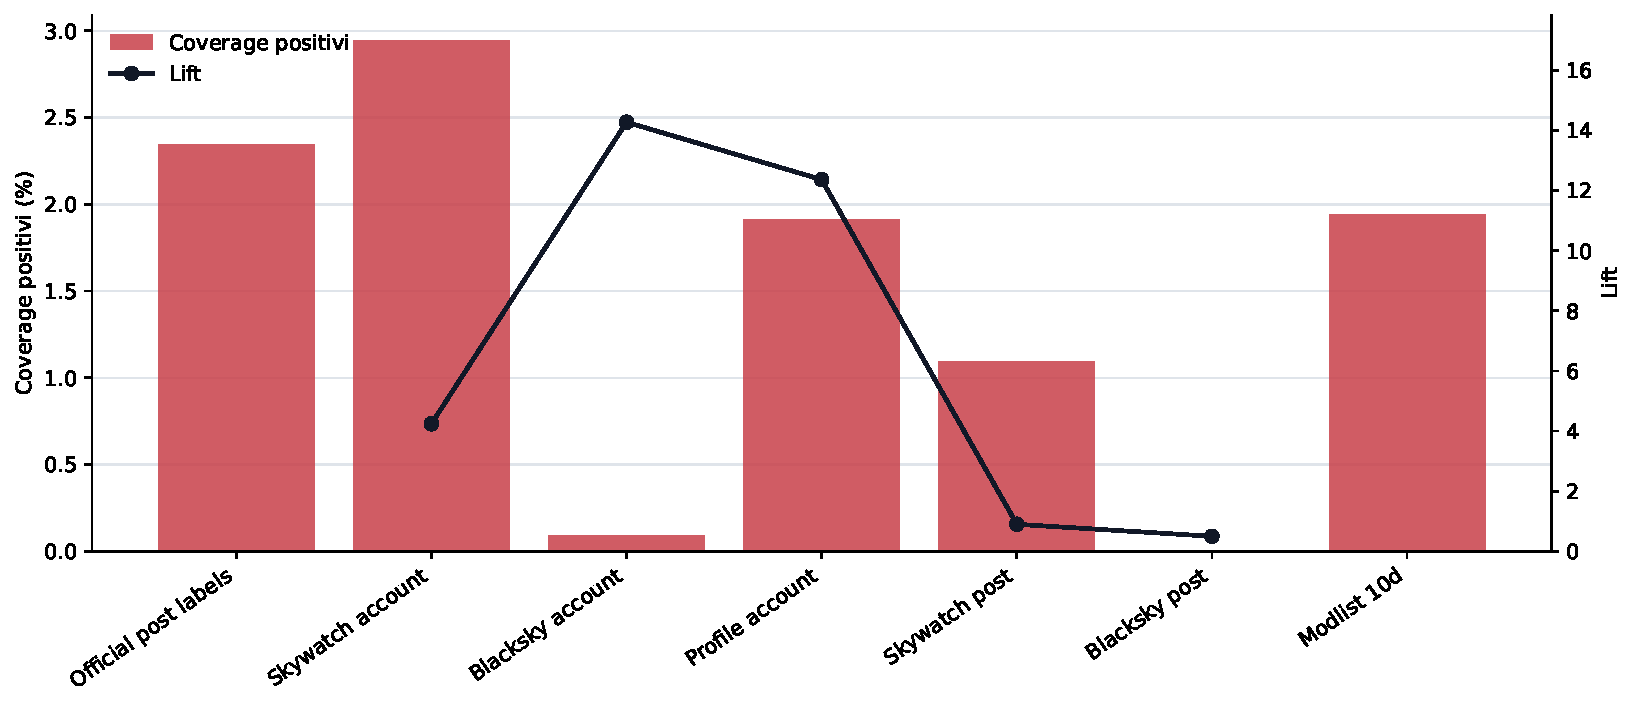
\includegraphics[width=\linewidth]{fig13_coverage_lift.pdf}
  \caption{Coverage e lift per labels, labeler terzi e modlist. Il lift elevato di alcuni segnali non compensa la bassa coverage.}
  \label{fig:coverage-lift}
\end{figure}

\FloatBarrier

\section{Discussione}

I risultati indicano che i blocchi ricevuti sono il segnale comunitario piu' informativo tra quelli analizzati, ma il loro potere dipende dall'esposizione pubblica dell'account. La distinzione centrale e' tra due regimi.

Nel regime degli account esposti, cioe' 0p, p0 e soprattutto pp, gli account sono osservabili dalla comunita', possono accumulare blocchi e mostrano un segnale temporalmente concentrato vicino al takedown. La Random Forest non produce una previsione completa, ma distingue parzialmente positivi e negativi: la precision e' alta, mentre la recall resta moderata. Questo profilo e' coerente con un segnale utile quando presente, ma incapace di coprire l'intera popolazione dei takedown. Il gruppo pp, che combina attivita' e visibilita', e' quello con maggiore separabilita' predittiva.

Nel regime del corner 00, molti positivi hanno zero post e zero follow ricevuti nella finestra osservata. Essi accumulano pochi blocchi in valore assoluto e spesso presentano lifetime molto breve. Questa dinamica e' coerente con account usa-e-getta, spam, ban evasion, impersonation o altri pattern anti-abuso account-level, ma il dataset non osserva direttamente la causa del takedown e non consente una classificazione sostantiva dei singoli account. L'interpretazione prudente e' che una quota rilevante di takedown ufficiali avvenga prima che un segnale comunitario pubblico possa formarsi.

La temporalita' del segnale e' particolarmente rilevante. Nei gruppi esposti, il giorno immediatamente precedente all'evento ha un peso elevato sia descrittivamente sia nella feature importance. Questo suggerisce una capacita' predittiva ravvicinata: i blocchi non anticipano necessariamente il takedown su orizzonti lunghi, ma contengono informazione nelle ore e nei giorni immediatamente precedenti. La previsione e' quindi utile in senso statistico e operativo limitato, non come sistema generale di early warning distante nel tempo.

Labels e modlist mostrano un risultato diverso. Alcuni labeler terzi hanno lift elevati, ma la coverage e' troppo bassa per sostenere una predizione sistematica. Questo non implica che i labeler siano teoricamente irrilevanti: possono servire nicchie specifiche, policy particolari o comunita' delimitate. Nel dataset operativo, pero', non coprono una quota sufficiente dei positivi pre-takedown. La stessa conclusione vale per le modlist, che rappresentano un segnale comunitario aggregato interessante ma raro nella finestra considerata.

Nel complesso, la moderazione comunitaria e quella ufficiale non appaiono come sistemi sovrapposti perfettamente. Per gli account esposti, i blocchi possono precedere temporalmente l'enforcement ufficiale e contenere informazione predittiva. Per molti account 00, l'enforcement ufficiale sembra invece agire su segnali account-level o anti-abuso non osservati pubblicamente. Il contributo principale del lavoro e' rendere empiricamente visibile questa eterogeneita'.

\section{Limiti}

\subsection{Validita' interna}

Il target \code{!takedown} e' un proxy imperfetto dell'enforcement ufficiale. Revoche e takedown multipli sono rari ma presenti; inoltre, la causa del takedown non e' osservata. I timestamp \code{created_at} possono avere anomalie o mancate disponibilita', specialmente nelle analisi di lifetime. Per i negativi, lo pseudo-event time controlla il calendario ma non equivale a un evento reale. Alcuni account negativi possono comparire in piu' osservazioni account-giorno, creando dipendenza tra righe. Di conseguenza, uno stesso DID potrebbe comparire in fold differenti nelle cross-validation se non viene applicata una grouped cross-validation.

Un limite importante riguarda la validazione predittiva: le metriche principali sono basate su predizioni out-of-fold in cross-validation e non su una validazione temporale esterna. Inoltre, il campionamento bilanciato impone una prevalenza artificiale del 50\%, diversa dalla prevalenza reale dei takedown nella popolazione osservabile.

\subsection{Validita' esterna}

L'analisi e' limitata a marzo 2026 e a una finestra operativa specifica. La piattaforma evolve rapidamente, le policy possono cambiare e campagne spam concentrate nel tempo possono influenzare la composizione dei takedown. La generalizzabilita' ad altri mesi, ad altre fasi di crescita di Bluesky o ad altri social network deve quindi essere verificata con validazione temporale esterna.

\subsection{Validita' di costrutto}

Post e follow ricevuti sono proxy incompleti dell'esposizione pubblica: non misurano impressions, ranking nei feed, quote esterne o visibilita' algoritmica. I blocchi sono un proxy della reazione comunitaria, ma possono riflettere conflitti sociali, campagne coordinate o preferenze individuali non necessariamente legate a violazioni. Labels e modlist hanno coverage limitata e finalita' eterogenee. Le violazioni account-level sono anch'esse eterogenee: spam, impersonation, ban evasion e contenuti problematici possono produrre traiettorie di segnale diverse.

\subsection{Validita' statistica}

Le distribuzioni dei blocchi sono zero-inflated e heavy-tailed. Alcuni bucket di esposizione hanno celle sottili, quindi i confronti cromatici nelle heatmap vanno letti come descrittivi e non come test di significativita'. Le feature giornaliere sono correlate tra loro; la impurity-based feature importance puo' distribuire importanza tra variabili ridondanti ed e' sensibile alla struttura delle feature. Le analisi presentate sono quindi associative e predittive, non causali.

\section{Conclusioni e sviluppi futuri}

Le quattro domande di ricerca ricevono una risposta convergente. Rispetto a RQ1, gli account successivamente sottoposti a takedown ricevono piu' blocchi dei controlli e il segnale e' fortemente concentrato negli ultimi giorni, soprattutto nel giorno immediatamente precedente all'evento. Rispetto a RQ2, il potere informativo dei blocchi dipende dall'esposizione: funziona meglio per account con post e/o follow ricevuti, mentre e' debole per il corner 00. Rispetto a RQ3, una Random Forest basata sui blocker unici consente una discriminazione parziale ma non completa, con F1 out-of-fold pari a \num{0.6878} e ROC AUC pari a \num{0.7604}. Rispetto a RQ4, labels ufficiali post-level, labeler di terze parti e modlist hanno coverage troppo bassa per sostenere un uso predittivo sistematico, anche quando il lift e' elevato.

Il messaggio centrale e' che i blocchi ricevuti costituiscono il segnale comunitario piu' informativo tra quelli analizzati, ma il loro potere predittivo dipende dall'esposizione pubblica dell'account. Il segnale e' forte e temporalmente concentrato per gli account che hanno avuto il tempo di interagire con la comunita', mentre non puo' spiegare i takedown rapidissimi degli account privi di post e follow ricevuti. Labels e modlist presentano talvolta lift elevati, ma una coverage insufficiente per sostenere una predizione sistematica.

Il contributo principale e' distinguere empiricamente due famiglie di takedown: quelli che lasciano segnali comunitari pubblici nella finestra pre-evento e quelli che avvengono prima che tali segnali possano formarsi. Questa distinzione aiuta a interpretare la moderazione su Bluesky come interazione tra segnali comunitari osservabili e sistemi ufficiali account-level non completamente osservabili.

Gli sviluppi futuri includono l'estensione a piu' mesi, una validazione temporale su periodi successivi, grouped cross-validation per DID, validazione indipendente del modello, curve precision-recall, calibrazione delle probabilita' e sensitivity analysis su finestre di 3, 5, 7, 10 e 14 giorni. Ulteriori analisi potrebbero modellare il tempo al takedown con approcci di sopravvivenza, studiare il grafo dei blocker, includere centralita' e reputazione dei blocker, analizzare separatamente il corner 00 e classificare le cause dei takedown. Per l'interpretabilita' del modello, permutation importance e, in futuro, SHAP potrebbero essere applicati come tecniche aggiuntive; SHAP non e' stato usato nell'analisi corrente.


\printbibliography

\end{document}
